% (c) 2017 Daniele Zambelli - daniele.zambelli@gmail.com
% 
% Tutti i grafici per il capitolo relativo alle equazioni
%

\begin{comment}

\newcommand{\assea}{% Retta con numeri messi a caso.
    \disegno{
    }
}

\end{comment}

\newcommand{\alberoequazioni}{% Retta con numeri messi a caso.
  \def \xo{0}
  \def \yo{0}
  \def \dx{6}
  \def \dy{2}
  \def \xa{\xo+\dx}
  \def \ya{\yo+\dy}
  \def \xb{\xo+\dx}
  \def \yb{\yo-\dy}
  \def \xc{\xb+\dx}
  \def \yc{\yb+\dy}
  \def \xd{\xb+\dx}
  \def \yd{\yb-\dy}
  \def \xco{2}
  \def \yco{.2}
  \def \angle{25}
  \disegno{
    \draw (\xo, \yo) node [left=+2mm] {\(Ax = B\)} 
      (\xo, \yo) .. controls (\xo+\xco, \yo+\yco) and (\xa-\xco, \ya-\yco) .. 
      (\xa, \ya)
      node [midway, above, rotate=\angle] {\(A \ne 0\)}
      node [right=+2mm] {\(\IS=\graffa{\dfrac{B}{A}}\)};
    \draw 
      (\xo, \yo) .. controls (\xo+\xco, \yo-\yco) and (\xb-\xco, \yb+\yco) .. 
      (\xb, \yb) 
      node [midway, below, rotate=-\angle] {\(A = 0\)};
    \draw 
      (\xb, \yb) .. controls (\xb+\xco, \yb+\yco) and (\xc-\xco, \yc-\yco) .. 
      (\xc, \yc) 
      node [midway, above, rotate=\angle] {\(B \ne 0\)}
      node [right=+2mm] {\(\IS=\emptyset\)};
    \draw 
      (\xb, \yb) .. controls (\xb+\xco, \yb-\yco) and (\xd-\xco, \yd+\yco) .. 
      (\xd, \yd) 
      node [midway, above, rotate=-\angle] {\(B = 0\)}
      node [right=+2mm] {\(\IS=\Q\)};
    \foreach \x/\y in {\xo/\yo, \xa/\ya, \xb/\yb, \xc/\yc, \xd/\yd}
      {\filldraw (\x, \y) [fill=blue] circle (2pt);}
  }
}

% \begin{tikzpicture}[x=5mm, y=5mm,font=\small]
% \tikzstyle{level 1}=[level distance=2cm, sibling distance=2.cm]
% \tikzstyle{level 2}=[level distance=2cm, sibling distance=1.cm]
% \tikzstyle{point} = [circle,minimum width=3pt,fill, inner sep=0pt]
% 
% \node[point, label=left:{$A\cdot x =B$}] (aer) at (0,0) {}[grow'=right]
% child {node[point, label=right:{$A\ne 0\to$ equazione determinata e 
% $\IS=\left\{\dfrac{B}{A}\right\}$}] {} 
% }
% child {node[point, label=below:{$A=0$}] {} 
% child {node[point,label=right:{$B=0\to$ equazione indeterminata e $\IS=\insQ$}] 
% {}}
% child {node[point,label=right:{$B\ne 0\to$ equazione impossibile e 
% $\IS=\emptyset $}] {}}
% } ;
% \end{tikzpicture}

\newcommand{\piattello}[2]{% disegna un piattello della bilancia
  \def \xv{#1}
  \def \yv{#2}
  \def \dxtop{2.6}
  \def \dytop{5.7}
  \def \dxbase{2.2}
  \def \dybase{6.1}
  \draw (\xv-\dxtop, \yv-\dytop) -- (\xv, \yv) -- (\xv+\dxtop, \yv-\dytop);
  \draw [very thick]
    (\xv-\dxtop, \yv-\dytop) 
    .. controls (\xv-\dxtop, \yv-\dybase) and (\xv-\dxtop, \yv-\dybase) .. 
    (\xv-\dxbase, \yv-\dybase) -- (\xv+\dxbase, \yv-\dybase)
    .. controls (\xv+\dxtop, \yv-\dybase) and (\xv+\dxtop, \yv-\dybase) .. 
    (\xv+\dxtop, \yv-\dytop) ;
}

\newcommand{\bilancia}{% Disegna una bilancia con i piattelli vuoti

\begin{scope}[fill=black, draw=black]
\filldraw (0,0) rectangle (4,1);
\filldraw[rounded corners=2] (1,1.1)rectangle (3,1.6);
\filldraw (1.8,1.7) rectangle (2.3,8);
\filldraw[rounded corners=2] (1.5,8.1)rectangle (2.6,8.6);
\filldraw (-4,8.7) rectangle (8,9.1);
\filldraw[rounded corners=2] (1.8,8.8)rectangle (2.3,9.8);

\piattello{-4}{8.7}

\piattello{8}{8.7}
\end{scope}
}

\newcommand{\bilance}{% Due bilance per un problema.

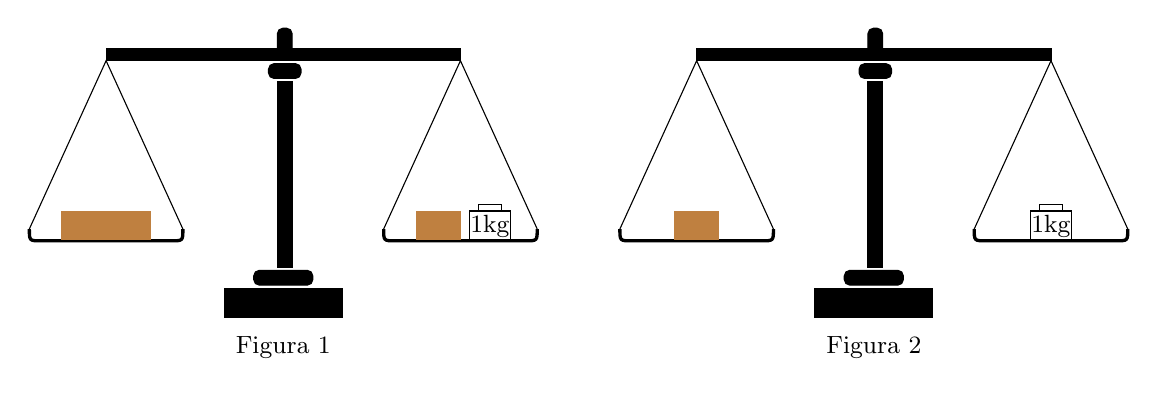
\begin{tikzpicture}[font=\small,x=5mm, y=5mm, scale=.75]
\bilancia
\filldraw[fill=brown, draw=brown](-5.5, 2.65) rectangle (-2.5, 3.6);
\filldraw[fill=brown, draw=brown](6.5,2.65) rectangle (8, 3.6);
\filldraw[fill=white] (8.3, 2.65) rectangle (9.7, 3.61);
\filldraw[fill=white] (8.6, 3.61) rectangle (9.4, 3.84);
\node () at (9, 3.1) {1kg};
\node () at (2,-1) {Figura 1};

\begin{scope}[xshift=100mm]
\bilancia
\filldraw[fill=brown, draw=brown](-4.75, 2.65) rectangle (-3.25, 3.6);
\filldraw[fill=white] (7.3, 2.65) rectangle (8.7, 3.61);
\filldraw[fill=white] (7.6, 3.61) rectangle (8.4, 3.84);
\node () at (8, 3.1) {1kg};
\node () at (2,-1) {Figura 2};
\end{scope}

\end{tikzpicture}

}

% \begin{tikzpicture}[font=\small,x=5mm, y=5mm, scale=.75]
% 
% \begin{scope}[fill=black, draw=black]
% \filldraw (0,0) rectangle (4,1);
% \filldraw[rounded corners=2] (1,1.1)rectangle (3,1.6);
% \filldraw (1.8,1.7) rectangle (2.3,8);
% \filldraw[rounded corners=2] (1.5,8.1)rectangle (2.6,8.6);
% \filldraw (-4,8.7) rectangle (8,9.1);
% \filldraw[rounded corners=2] (1.8,8.8)rectangle (2.3,9.8);
% 
% \node[name=c1,shape=semicircle,shape border rotate=180, inner 
% sep=3.75mm,draw=black, fill=black] at (-4,3)
% {};
% \node (a) at (-4,8.7) {};
% \draw (a.center)--(c1.arc start);
% \draw (a.center)--(c1.arc end);
% 
% \node[name=c2,shape=semicircle,shape border rotate=180, inner 
% sep=3.75mm,draw=black, fill=black] at (8,3)
% {};
% \node (b) at (8,8.7) {};
% \draw (b.center)--(c2.arc start);
% \draw (b.center)--(c2.arc end);
% 
% \filldraw[fill=orange, draw=orange](-5.5,4.02) rectangle (-2.5,5.1);
% \filldraw[fill=orange, draw=orange](6.5,4.02) rectangle (8,5.1);
% \filldraw[fill=white] (8.3,4) rectangle (9.7,5.1);
% \filldraw[fill=white] (8.6,5.1) rectangle (9.4,5.4);
% \node () at (9,4.5) {1kg};
% \node () at (2,-1) {Figura 1};
% \end{scope}
% 
% \begin{scope}[fill=black, draw=black, xshift=100mm]
% \filldraw (0,0) rectangle (4,1);
% \filldraw[rounded corners=2] (1,1.1)rectangle (3,1.6);
% \filldraw (1.8,1.7) rectangle (2.3,8);
% \filldraw[rounded corners=2] (1.5,8.1)rectangle (2.6,8.6);
% \filldraw (-4,8.7) rectangle (8,9.1);
% \filldraw[rounded corners=2] (1.8,8.8)rectangle (2.3,9.8);
% 
% \node[name=c1,shape=semicircle,shape border rotate=180, inner 
% sep=3.75mm,draw=black, fill=black] at (-4,3)
% {};
% \node (a) at (-4,8.7) {};
% \draw (a.center)--(c1.arc start);
% \draw (a.center)--(c1.arc end);
% 
% \node[name=c2,shape=semicircle,shape border rotate=180, inner 
% sep=3.75mm,draw=black, fill=black] at (8,3)
% {};
% \node (b) at (8,8.7) {};
% \draw (b.center)--(c2.arc start);
% \draw (b.center)--(c2.arc end);
% 
% \filldraw[fill=orange, draw=orange](-5,4.02) rectangle (-3,5.1);
% \filldraw[fill=white] (7.3,4) rectangle (8.7,5.1);
% \filldraw[fill=white] (7.6,5.1) rectangle (8.4,5.4);
% \node () at (8,4.5) {1kg};
% \node () at (2,-1) {Figura 2};
% \end{scope}
% 
% \end{tikzpicture}

\newcommand{\rettangolo}{% Retta con numeri messi a caso.
    \disegno{
\draw (0, 0) node [below left] {\(A\)} --
      (7, 0) node [below right] {\(B\)} -- 
      (7, 4) node [above right] {\(C\)} -- 
      (0, 4) node [above left] {\(D\)} -- cycle;
    }
}

% \begin{tikzpicture}[font=\small,x=8mm, y=3.5mm]
% 
% \draw (0,0) rectangle (4,4);
% 
% \begin{scope}[left]
% \node  at (0,4) {$A$};
% \node  at (0,0) {$D$};
% \end{scope}
% 
% \begin{scope}[right]
% \node  at (4,4) {$B$};
% \node  at (4,0) {$C$};
% \end{scope}
% \end{tikzpicture}

\newcommand{\triangolo}{% Retta con numeri messi a caso.
    \disegno{
\draw (0, 0) node [below left] {\(A\)} --
      (7, 0) node [below right] {\(B\)} -- 
      (0, 4) node [above left] {\(C\)} -- cycle;
    }
}

% \begin{tikzpicture}[font=\small,x=5mm, y=5mm]
% 
% \draw (0,0)-- (4,0)--(0,3)--(0,0);
% 
%  \begin{scope}[left]
% \node  at (0,3) {$C$};
% \node  at (0,0) {$A$};
% \end{scope}
% 
% \node[right]  at (4,0) {$B$};
% 
% \end{tikzpicture}

% 
% \begin{hieroglyph}
% D34\s1
% \end{hieroglyph}.
% 
% \begin{hieroglyph}
% {\leavevmode \loneSign{{\Hsmaller\Aca GD/66/}}}
% \end{hieroglyph}.

